\section{Program manual}
\label{Sec.FortranProgram}

This is Fortran-base open-source software, which can be downloaded from: {\tt https://wiki-zeuthen.desy.de/HERAverager}. Installation and basic pre-requirements are described in Sec.~\ref{Sec:Install}. Code organization is shown in Sec.~\ref{Sec:Code}.

The input and output formats are explained in Sec.~\ref{Sec:Input} and Sec.~\ref{Sec:Output} respectively.

\subsection{Program installation}
\label{Sec:Install}
The program requires gfortran compiler to be compiled.

The program can be unpacked and installed with following lines:
\begin{verbatim}
    tar -xvzf heraverager-1.0.0.tar.gz
    cd heraverager-1.0.0
    autoreconf --install
    ./configure
    make 
    make install
\end{verbatim}

After successful installation an executable file can be found in: {\tt ./bin/HERAverager }. All input parameters are defined in the steering file. Test run of the program, using test steering file (is in {\tt ./test/steering}) can be performed with lines:

\begin{verbatim}
    cd ./bin
    ./HERAverager ../test/steering
\end{verbatim}

The output information is located in {\tt ./output/}

\subsection{Code organization}
\label{Sec:Code}

Package consist of following subdirectories:

\begin{itemize}
\item {\tt include}: include-file with declaration of global variables
\item {\tt source}: source-code files
\item {\tt doc}: documentation to the program, including this manual.
\item {\tt test}: example of steering and data files
\item {\tt num\_utils}: Utilities for the averaging.
\end{itemize}

Short description of source files is given below:

\begin{itemize}
\item {\tt averaging.f}: Calling functions to prepare arrays and perform the combination   
\item {\tt average\_py.f90}: Interface to python (see Sec.~\ref{sec:python})
\item {\tt error\_logging.f}: print full error summary and close files
\item {\tt initave.f}: Reading the data and preparing for the combination
\item {\tt statrecalc.f}: Recalculate systematic uncertainties after combination and prepare values for the next iterator. 
\item {\tt common\_tools.f}: Function, used in different steps of the combination 
\item {\tt fillarrays.f}: Prepare arrays used for combination
\item {\tt output.f}: Print output of the combination in output files
%\item {\tt swimming.f}
\item {\tt covartonui.f}: Convert covariance matrix to nuisance param. representation
\item {\tt heraverager.f}: Main file, which is calling functions for initialization, combination and output.
\item {\tt readdata.f}: Read a table of measurement with their uncertainties from single experiment
\item {\tt toblockdiag.f}: Perform the combination by minimization of linearised $\chi^2$
\end{itemize}

Summary of the code structure is shown in Fig.~\ref{fig:code}. 3 logic blocks: initialization, combination and output are encapsulated in 3 functions called in {\tt heraverager.f}.

At initialization step all files with data and options are read and values are stored in global internal variables. First code read the steering file, which contain all options of the combination and list of data files. During the loop over data files the name of systematic sources, values of the measurements and their uncertainties are stored in global variables.

Combination block have a loop over all off-set systematics (2N+1 times, see Sec.~\ref{Sec:offset}) and over iterations. Combination process starts with filling of auxiliary arrays (mainly elements of Eq.~\ref{Eq:MatrixEQ}). Then minimization is performed and results are stored in global internal variables. In case if it was not the last iteration statistical and systematic uncertainties are recalculated (See Sec.~\ref{Sec:MinimizeBias}).

The output written in different files. Systematic uncertainties can be presented in different ways (See Sec.~\ref{Sec:SystRepresentation}), depending on options in the steering file.


\begin{figure}
  \centering
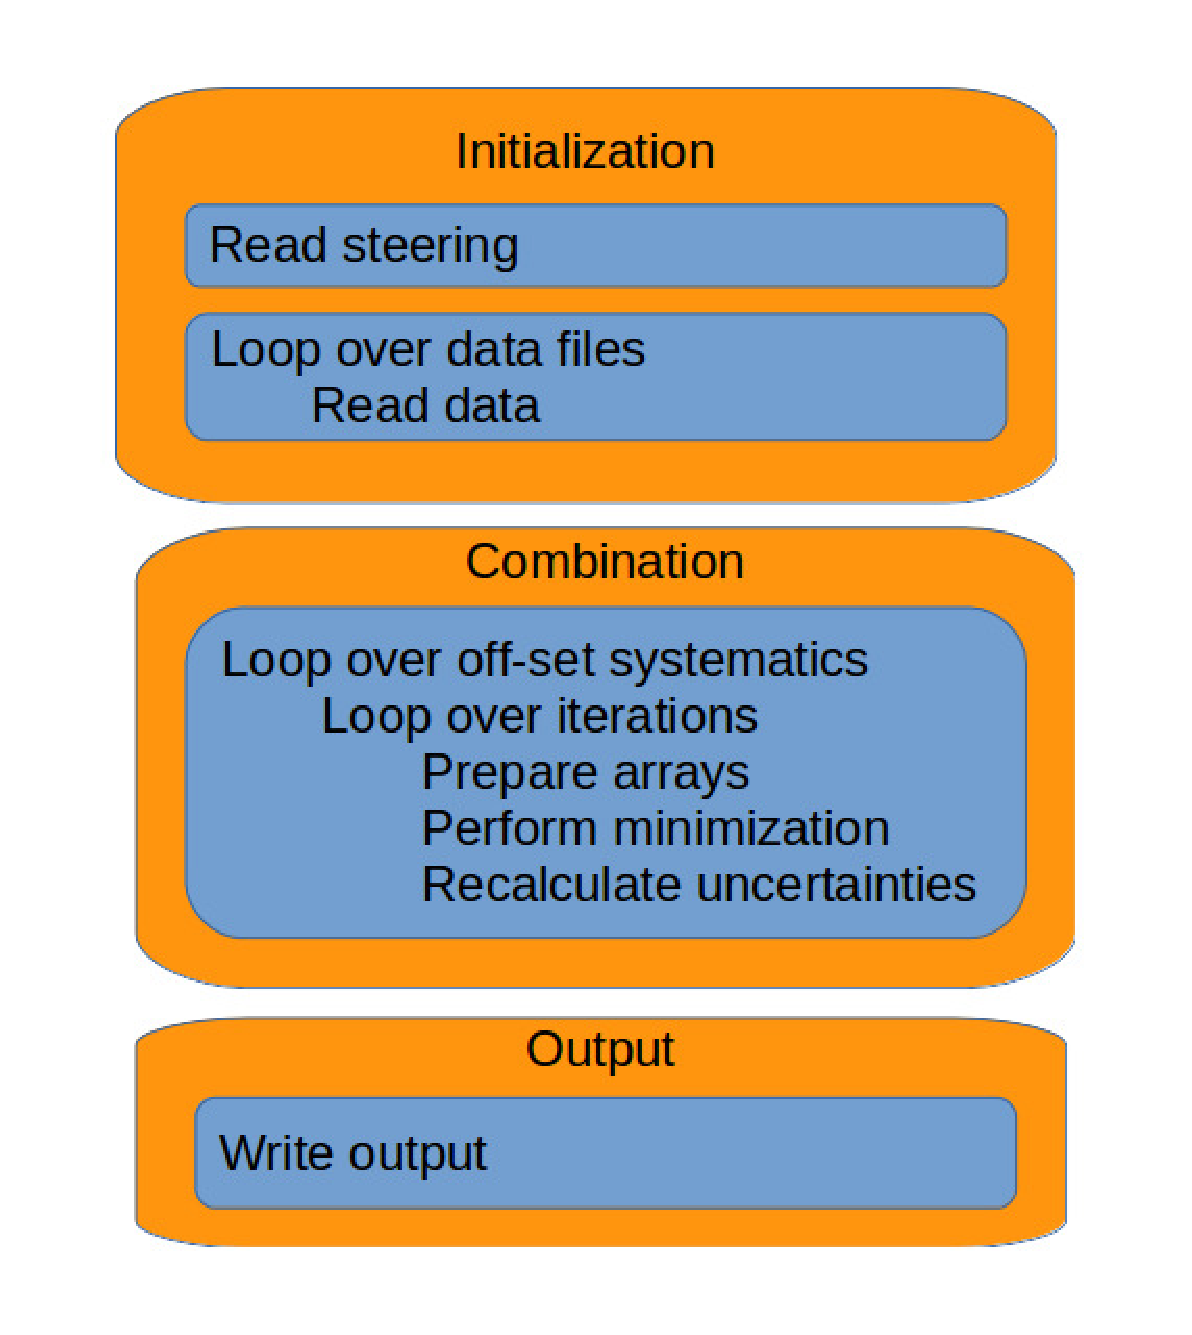
\includegraphics[width=0.65\linewidth]{figures/code.pdf}
  \caption{Code organization of the combination tool.}
  \label{fig:code}
\end{figure}


\subsection{Input information}
\label{Sec:Input}

All input of the combination as well as the list of data files and supplementary information is given in the steering file. The description of the steering file in given in Sec.~\ref{Sec:Steerign}, while data file is discussed in Sec.~\ref{Sec:Data}.

\subsubsection{Steering file}
\label{Sec:Steerign}

Steering file is organized in blocks, which corresponds to name-lists in the Fortran code. Lines, which starts with ! are commented. Structure and meaning of these blocks are described below:

\begin{verbatim}
&InFiles
  ! Specify data files to be averaged
  NInputFiles = 2
  InputFileNames(1) = '../test/h1460new.public.dat'
  InputFileNames(2) = '../test/zeus460.public.dat'
&End
\end{verbatim}
Block contains the list of data-files (see structure of the data files in Sec.~\ref{Sec:Data}). Path to these files have to be absolute and relative with respect to the place, where the program runs.


\begin{verbatim}
&CommonGrid
  GridType = 'External' !  'External' or 'Auto'
  GridFiles = '../test/grid460575.dat'
  AveSameExp = .true.
&End
\end{verbatim}
Most of the measurements, for which tool is designed are binned measurements. The binning can be taken directly from the data file (option {\tt 'Auto'}) or can be written externally (option {\tt 'External'}) in grid of bins. 

In case of external binning, files which describe binning have to be provided and have structure, similar to:

\begin{verbatim}
&Grid
  Reaction = 'NC e+-p'
  NDimension = 2
  NPoints = 630
  BinNames = 'Q2','x'
&End
  1.5  0.000378678
  1.5  0.000227206998
  1.5  0.000134258007
  1.5  9.52802002E-05
\end{verbatim}
Where:
\begin{itemize}
\item {\tt Reaction} is the name of measured process
\item {\tt NDimension} is the number of dimensions of the binning
\item {\tt NPoints} total number of bins
\item {\tt BinNames} name of the dimensions.
\end{itemize}

Numbers below the header define the center of bins. Each line represent one bin (number of lines should be equal to the total number of bins). Number of columns corresponds to the number of dimensions (two in this example) and define center of bins in each dimension ('Q2' and 'X' in example).

Each grid-file describe the binning for a certain measured process (reaction). In case of combination of the data for several different processes, several grid files have to be given.

The name of dimensions and the name of measured process should coincide with one given in data file (see Sec.~\ref{Sec:Data}). The measurements are considered as a measurements of the same physics quantity if bins, bin names and reactions are coincides. 

In case if the bin-centers in the data file are different compared to bin-centers in the grid file nearest bin of the grid file will be used to define the bin. Parameter {\tt AveSameExp} clarifies, how to treat the case when two bins from one experiment go to one grid bin:
\begin{itemize}
\item {\tt .true.} - weighted average of these bins will be used for combination.
\item {\tt .false.} - measurements in these bins will be combined as different measurements of the same physics quantity.
\end{itemize}

\begin{verbatim}
&HERAverager
  OutputMode  = 'ORTH'
  OutputPrefix = 'Ave' 
  OutputFolder = '../output'   
  IDebug = 0
  WriteOriginal = .false.
  WriteSysTexTable = .false.
  PostRotateSyst = .true.
&End
\end{verbatim}

{\tt OutputMode} - is the output options for the systematics uncertainties (see Sec.~\ref{Sec:SystRepresentation}).
\begin{itemize}
\item {\tt 'ORTH'} - orthogonal representation
\item {\tt 'ORIG'} - original structure of the systematic uncertainties.
\end{itemize}

{\tt OutputPrefix} Add a prefix for output file names

{\tt OutputFolder} - folder, where the output information is stored

{\tt PostRotateSyst = .true.} keep output systematic uncertainties align to the original sources as much as possible.

{\tt IDebug} - Debug level. Higher value corresponds to more debug messages.

{\tt WriteOriginal} - include original information to the output summary (file {\tt ave Ave.dat}, see Sec.~\ref{Sec:Output}) 

{\tt WriteSysTexTable} - write output information about systematic uncertainties in tex format (file {\tt sys.tex}, see Sec.~\ref{Sec:Output})

\begin{verbatim}
&BiasCorrection
  AverageType = 'MIXED'
  Iteration = 10
 ! Rescale the stat and uncorr uncertainties separately:
  RescaleStatSep = .false.
 ! Correction of the syst bias for stat errors
  CorrectStatBias = .false.
 ! Keeping the stat errors fixed'
  FixStat = .false.
&End
\end{verbatim}
Parameter {\tt AverageType} define the type of the systematic uncertainties
\begin{itemize}
\item {\tt 'ADD'} - all systematic uncertainties are processed as additive
\item {\tt 'MULT'} - all systematic uncertainties are processed as multiplicative
\item {\tt 'MIXED'} - type of systematic uncertainties is taken from the data file
\end{itemize}

Parameter {\tt Iteration} set the number of iterations. In case, if all uncertainties are additive and symmetric $\chi^2$ is linear, no additional iteration is required. In case of multiplicative systematic uncertainties 2-3 iterations are recommended to get stable combined value. If some of the uncertainties are asymmetric number of iteration have to increased (7-10 iterations).

Correction of the statistical uncertainties, discussed in Sec.~\ref{Sec:StatBias} is normally performed for both statistical and uncorrelated systematic uncertainties. This correction can be done separately for each of therm by setting flag {\tt RescaleStatSep = .true.}. Using flag {\tt FixStat = .false.} statistical uncertainties are still uncorrected.

Setting flag {\tt CorrectStatBias = .true.} statistical bias is corrected by implementing Eq.~\ref{Eq:StatCorr2}


\subsubsection{Data file}
\label{Sec:Data}

The data-file is an ascii-file, which contains measurement values in a certain bins and their uncertainties. 

The data file consist of the header and lines of data:
\begin{verbatim}
 &Data
   Name = 'H1' 
   NData = 72
   NColumn = 9
   ColumnType = 2*'Bin','Sigma', 6*'Error' 
   ColumnName = 'Q2', 'x', 'x-sec', 'stat', 'uncor','sys1','sys2:O','sys3+','sys3-'
   Reaction = 'NC e+-p' 
                                                     
   Percent = true,true,true,true,true,true
                                                     
 &END
   1.500  3.47999E-05  0.51952   8.10   4.96  0.69  8.00  0.45   0.58   
   2.000  4.64000E-05  0.70449   4.57   4.31  1.10 -0.81  0.49   0.59
\end{verbatim}

Header of the data file contain following information:

\begin{itemize}
\item {\tt Name}: A name of the data file, which is used for user-friendly output
\item {\tt NData}: Number of data points (bins)
\item {\tt NColumn}: Total number of columns in the table, which includes bins, value of the measurement and uncertainties
\item {\tt ColumnType}: Type of the column. In case if several columns have the same type they can be grouped as e.g. {\tt 6*'Error'}. All columns should have a type. Following types are supported:
\begin{itemize}
\item {\tt Bin}: Bin-center. Number of these columns gives the number of dimensions of the measurement.
\item {\tt Sigma}: Value of the measurement  
\item {\tt Error}: Uncertainty
%\item {\tt ignore}: column is ignored
\end{itemize}
\item {\tt ColumnName}: The name of the column. All columns should have a name. In case of 'Bin' type of the column name specify the name of the dimension. If case of using external grid file these names have to be mentioned in the grid file. For the 'Error' type of the column the name specify the name and type of systematic uncertainty. Following type of systematic uncertainties are supported:
\begin{itemize}
\item {\tt stat}: Statistical uncertainty
\item {\tt uncor}:  Bin-to-Bin uncorrelated systematic uncertainty
\item {\tt ignore}: Column ignored
\item {\tt somename}: Bin-to-Bin correlated multiplicative systematic uncertainty with the name ``somename''. One data-file should not contain two columns with uncertainties with the same names. If systematic uncertainty with the same name is found in different data-files, they are considered as correlated between measurements.
\item {\tt somename:O}: Off-set systematic uncertainty
\item {\tt somename:A}: Bin-to-Bin correlated additive systematic uncertainty
\item {\tt somename+}, {\tt somename-}: Bin-to-Bin correlated asymmetric systematic uncertainty (can be {\tt :0} or {\tt :A}). Each asymmetric systematic uncertainty should contain both + and - part. 
\end{itemize}
\item {\tt Reaction}: is the name of measured process. In case of using external grid file this name have to be mentioned in the grid file.
\item {\tt Percent}: Array of flags, shows is corresponding uncertainty is given in \% or absolute. Number of entries in this field should corresponds to the number of uncertainties. 

\end{itemize}

The data are given below the header as a table. The structure of the table corresponds to one described in the header. In a given example the table should contain 72 rows and 9 columns.

\subsection{Output information}
\label{Sec:Output}

Output information are stored in ascii files inside of output folder. If this folder does not exist, the folder will be created automatically. If the files with the same names are exists, they will be overwritten.

output information consist of following files:
\begin{itemize}
\item {\tt matrix.dat}: Covariance matrix $\Gamma_{ave}$
\item {\tt eigvalues.dat}: Eigenvalues of matrix $\Gamma_{ave}$
\item {\tt eigvectors.dat}: Eigenvectors of matrix $\Gamma_{ave}$

\item {\tt tab.dat} -- Summary table of the combination: combined value, statistical uncertainty, uncorrelated systematic uncertainty, all sources of the correlated systematic uncertainties.
\item {\tt ave\_Ave.dat}: -- Short summary of the combination: Bin centers, combined value, statistical uncertainty, total systematic uncertainty, total uncertainty 
\item {\tt ave\_proc\_Ave101.dat} -- Summary of the combination, in the format of data file.
\item {\tt sys.txt} -- Shift and reduction of the systematic uncertainties: count-number of systematic uncertainty, name of systematic uncertainty, shift of systematic $\beta_{i,ave}$ (see Eq.~\ref{Eq:AveMu}), reduction of the systematic uncertainty $D_{jj}$ (see Eq.~\ref{Eq:Diag}), pull of systematic uncertainty (see Eq.~\ref{Eq:PullSyst}).
\item {\tt sys.tex} same as {\tt sys.txt}, but in latex format
\item {\tt chi2map.dat} -- Information about pulls (see Eq.~\ref{Eq:Pulls}). The information is given in a table with columns: Count-number of the data point, number of degrees of freedom, bin1, .., binN, pull, data-file.
\item {\tt offsettab.dat} -- Summary of off-set systematic uncertainties: combined value for all iterations over offset systematics (see Sec.~\ref{Sec:offset})
\item {\tt ItrInfo.dat} -- Information about systematics shifts and $\chi^2$ compatibility for all performed iterations. First line shows $\chi^2$, other lines show systematic shifts for different systematic sources. Different columns show values for different iterations.  
\end{itemize}




  